%==============================================================================
% 七、问题二的模型建立与求解
%==============================================================================
\section{问题二：关键化合物的归因}

\subsection{建模思路}

问题二要求给出每个感官项最关键的三类化合物，并论证结果稳定、化学上讲得通。建模前须先排除两条看似可行的捷径。

第一条是直接采用附件8 的现成排序。该文件已提供 MDI 与 SHAP 两张化合物重要性表，取用最省力，但不适用：二者是全部 231 列对某一个综合目标的排序，并非对 50 个感官项分别排序；且重要性只说明模型在多大程度上用到了该列，不说明因果关系\cite{lundberg2017}。本文只把这两张表留作事后方向对照。

第二条是逐列计算重要性。231 个指标中有 219 个的方差膨胀因子大于 10，而相关系数绝对值超过 0.9 的只有 6 对，说明共线是一大片弱相关的累积而非少数几列重复。此时逐列打乱，被打乱的列会被同族其余列顶替，算出的重要性系统性偏小\cite{strobl2008}。

排除这两条之后，本问的技术路线分四步：先诊断附件2 的化合物网络能否直接用于分组；再用\emph{逐列置换重要性}配合 \emph{LightGBM} 完成候选排序；用\emph{自助重采样} 200 次量化稳定性；最后用\emph{气味活性值}作化学裁判。

\subsection{化合物网络的结构诊断}

题面要求以附件2 建立化合物共表达图。本文先按 $|\rho|\geq\tau$ 阈值化后取组合拉普拉斯 $L=D-A$，做特征分解并在前 $k$ 个特征向量上跑 \emph{Ng--Jordan--Weiss 谱聚类}($k=12$)，再计算模块内与模块间的平均 $|\rho|$。这张矩阵已与附件1 的 Spearman 相关逐格复核：231 个节点中 212 个可经附件8 的化学名—字段名对照表对应到本文的 231 维特征，44732 个可比对格子的中位绝对差为 $8.33\times10^{-17}$，说明矩阵本身没有读错。

按原设定做下去会得到“社区结构很弱”的结论。本文复查后认为这个判断不成立，原因分三层。

第一层是实现问题。谱聚类用纯随机初始化时，在这张图上收敛到退化解——231 个节点里有 79\%(183 个)被并进同一个“模块”。一个吞掉八成节点的划分，模块内与模块间自然拉不开差距，1.56 这个数字度量的是退化程度，不是图的结构。

第二层是方法问题。换成标准 Ng--Jordan--Weiss 所用的归一化拉普拉斯 $L_{\mathrm{sym}}=I-D^{-1/2}AD^{-1/2}$ 并加上 k-means++ 重启后，退化明显缓解，最大模块占比由 0.79 降到 0.38，但该划分的模块度仍只有 $-0.0034$。可见问题不在初始化，而在谱聚类本身：它以固定簇数 $k=12$ 切分，在密度 14.7\% 的稠密图上，前 12 个特征向量并不携带社区信息。

第三层才是图本身的结论。改用直接优化模块度的 \emph{Louvain 算法}，得 9 个社区、$Q=0.3229$，而 50 次度保持随机图的 95 分位为 0.2501，超出 0.0728；七个阈值下 $Q$ 均高于零分布，可见社区结构真实存在。三种聚类方式的定量对照见表~\ref{tab:q2graph}，模块度检验与模块内外相关性的对比见图~\ref{fig:q2graph}。

\begin{table}[htbp]
\centering
\footnotesize
\setlength{\tabcolsep}{3.5pt}
\caption{化合物网络的三种聚类方式对照。$\tau$ 为边阈值，$Q$ 为模块度}
\label{tab:q2graph}
\begin{tabular*}{\textwidth}{@{\extracolsep{\fill}}cccccc@{}}
\toprule
$\tau$ & \textbf{边数} & \textbf{原谱聚类：最大模块 / 内间比} & \textbf{归一化 $L$：最大模块 / $Q$} & \textbf{Louvain $Q$} & \textbf{零分布 95\%} \\
\midrule
0.10 & 15855 & 0.88 / 1.69 & 0.19 / $-0.0039$ & 0.0822 & 0.0538 \\
0.15 & 11642 & 0.80 / 1.58 & 0.17 / $-0.0039$ & 0.1359 & 0.0943 \\
0.20 & 8323  & 0.79 / 1.50 & 0.32 / $-0.0036$ & 0.1872 & 0.1397 \\
0.25 & 5739  & 0.60 / 1.50 & 0.28 / $-0.0036$ & 0.2474 & 0.1900 \\
0.30 & 3918  & 0.79 / 1.56 & 0.38 / $-0.0034$ & 0.3229 & 0.2501 \\
0.40 & 1660  & 0.38 / 1.42 & 0.47 / $-0.0032$ & 0.4831 & 0.3911 \\
0.50 & 645   & 0.58 / 1.67 & 0.61 / $-0.0026$ & 0.6513 & 0.5453 \\
\bottomrule
\end{tabular*}
\end{table}

\begin{figure}[htbp]
\centering
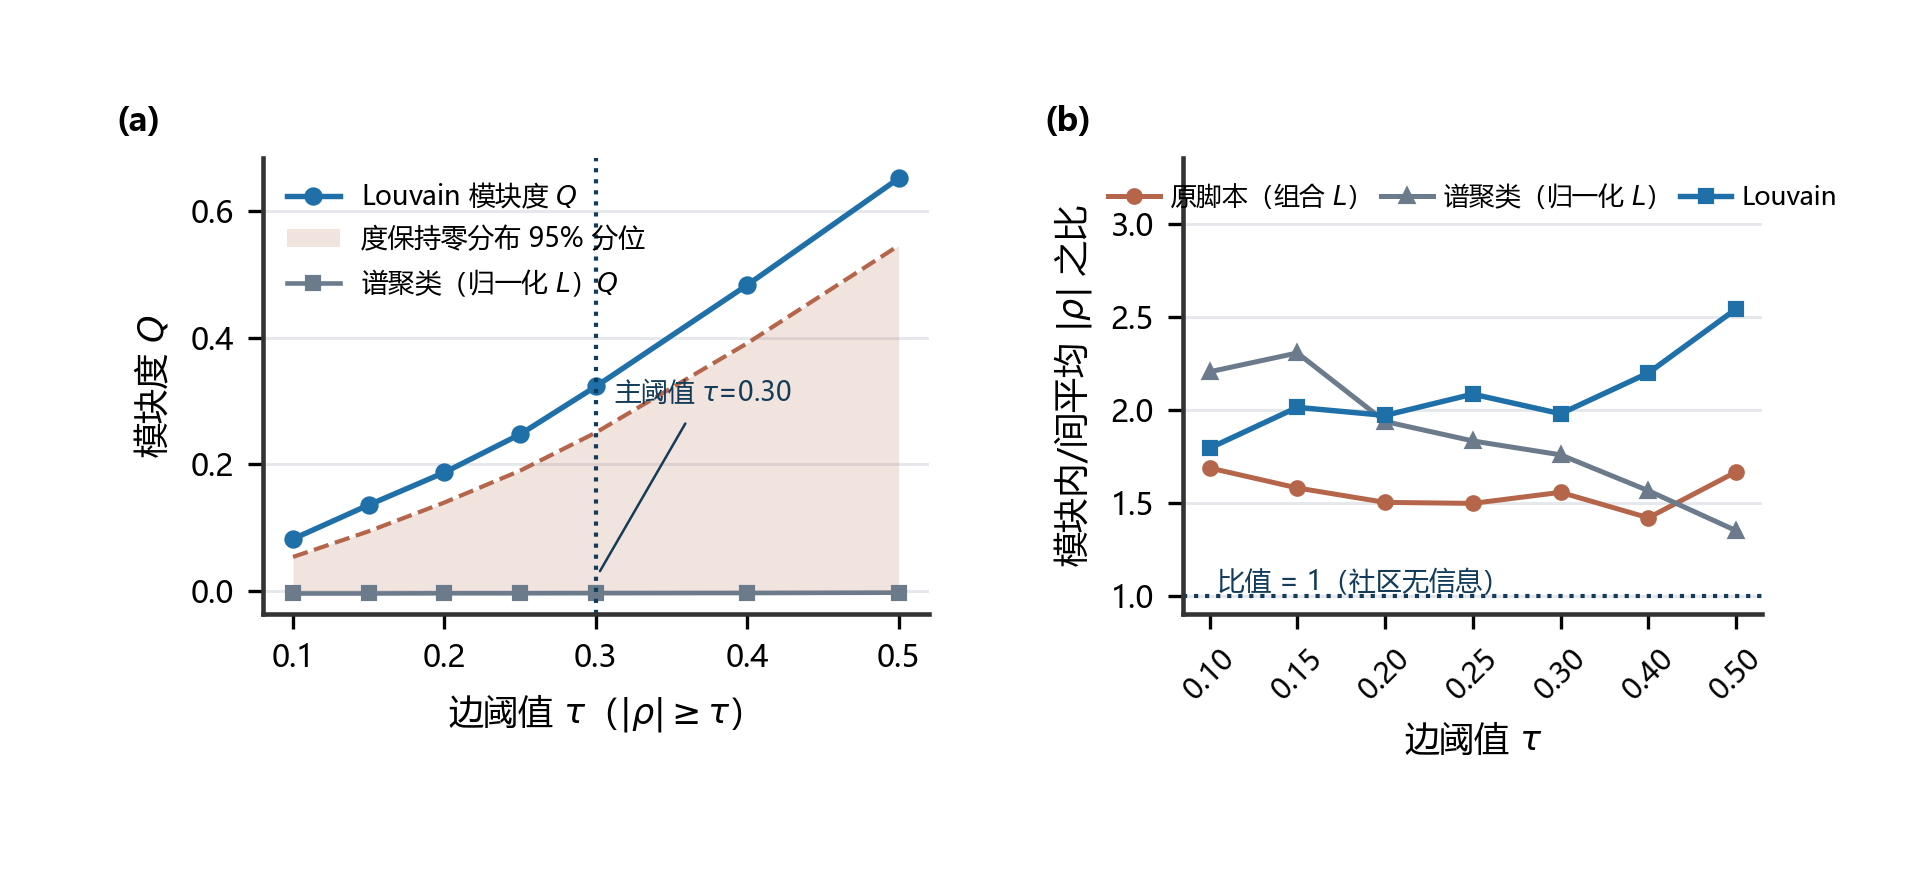
\includegraphics[width=0.79\textwidth]{figures/fig_q2_graph.png}
\caption{化合物网络的结构诊断。左图为 Louvain 模块度与度保持零分布，右图为三种聚类方式的模块内外 $|\rho|$ 对比}
\label{fig:q2graph}
\end{figure}

但这些社区不能直接用来做归因。把 Louvain 的 9 个社区与附件8 的化学来源分组对照，二者的调整兰德指数仅 0.0838、调整互信息仅 0.1109；反过来把化学族直接当作社区划分，模块度只有 0.0533。换言之，数据给出的社区与化合物来源几乎无关。同时 9 个社区覆盖 231 个节点、最大社区占 25\%，每个“模块”约 25 个化合物——用它做 Top-3 归因，等于先把 25 个化合物捆成一个不可拆的组，无法回答“哪 3 个最关键”这一题意。

因此本文的取舍是：附件2 的图用于结构诊断与特征预筛，归因的分组单位取附件8 的化学来源标注。三条理由都可量化：社区在统计上真实，$Q$ 高于零分布；在化学上不可解释，ARI 仅 0.0838；在粒度上不可用，约 25 个一组。

归因所用的分组来自附件8：231 个特征全部落在 7 族内，酵母代谢产物 78 个、酒花来源 77 个、其他 25 个（含 5 个派生总量）、香料陈化 23 个、麦芽 21 个、野生菌群 6 个、内标 1 个。这一划分有化学依据，且与前述共线结构相容——同族的弱相关累积正是共线的来源。

\subsection{逐列置换重要性与入选频率模型}

置换重要性的定义是“打乱某一列后预测性能掉多少”。逐列打乱有一个已知的缺陷：被打乱的列可以由同族的其他列顶上，掉幅被系统性低估\cite{strobl2008}。整族同时打乱可以避开这个偏差，但整族只给出 7 个族级数值，无法直接落成化合物排名——族内数十列共享同一个族级数值，要拆到单列只能按人为比例摊派，而摊派方式本身决定排名。本问要交付的是单个化合物的 Top-3，因此取逐列置换，族标签只用于汇报分组归属，不用于整组打乱。

本文对 50 个感官项分别建立 \emph{LightGBM 回归器}，在第 $b$ 次自助重采样的袋外样本上先算逐列置换重要性
\begin{equation}
  \Delta^{(b)}_{j}=R^{2}\left(\text{原样}\right)-R^{2}\left(\text{打乱第 }j\text{ 列}\right),
\end{equation}
再统计它进入前 10 名的频率
\begin{equation}
  \pi_{j}=\frac{1}{B}\sum_{b=1}^{B}\mathbf{1}\left[j\in\mathrm{Top10}\left(\Delta^{(b)}\right)\right],
  \qquad B=200,
\end{equation}
得到的是\emph{入选频率}而非单次重要性：单次 $\Delta^{(b)}_{j}$ 的噪声大到会反复变号，而 $\pi_j\in[0,1]$ 表示该列在 200 次重采样中稳居前 10 的比率，可以直接横向比较。第 $s$ 个感官项的 Top-3 取 $\pi_j$ 最大的三列构成 $\mathcal{T}_s$。由于实现上并未整族打乱，Top-3 应理解为模型相关性候选，不宜解释为独立的因果效应。

阈值由稳定选择的有限样本界反解。该界为 $\mathbb{E}[V]\le q_{\mathrm{sel}}^{2}/\left((2\pi_{\mathrm{thr}}-1)p\right)$，其中 $V$ 为误选变量数、$q_{\mathrm{sel}}$ 为基础选择程序每次选出的变量数、$p$ 为候选变量数。本文取 $q=1$、$p=231$，得
\begin{equation}
  \pi_{\mathrm{thr}}=\frac{1+q/p}{2}=0.5022 .
\end{equation}
这里 $q=1$ 的含义是“允许期望误选 1 个变量”，属操作性标准，\emph{不构成} 0.05 水平上的错误发现率控制——若严格按界中 $q_{\mathrm{sel}}$ 的原义取基础程序的选出数 10，同一式给出 0.7165，本文未采用。因此下文只称 $\pi_{\mathrm{thr}}$ 为入选频率阈值，不主张理论保证的错误发现率控制。

化学合理性用\emph{气味活性值}判断。对化合物 $j$ 与感官项 $i$，定义
\begin{equation}
  O_{ij}=\frac{c_{ij}}{T_j},
\end{equation}
$T_j$ 取自附件8 的香气阈值表，按单位分域处理(30 个阈值在 $\log_{10}$ 域、13 个在线性域，分别与浓度同域相除，不混用)。$O_{ij}>1$ 表示该化合物在样本中的浓度已超过其香气阈值，具备被感知的物质基础。据此把 150 条 Top-3 记录分为四档，判据只依赖阈值能否计算，不叠加显著性——显著性由 $\pi_{\mathrm{thr}}$ 单独把关：A 档阈值可算且 $O_{ij}\geq1$，浓度已超香气阈值；B 档阈值可算且 $0.5\leq O_{ij}<1$，接近阈值；C 档阈值可算但 $O_{ij}<0.5$，远低于阈值；N 档阈值缺失（表中无该化合物，或有行但阈值为 NA），OAV 不可算。

跨模型的稳定性用 \emph{Jaccard 系数}度量
\begin{equation}
  J\left(\mathcal{T}_s^{\,A},\mathcal{T}_s^{\,B}\right)
  =\frac{\left|\mathcal{T}_s^{\,A}\cap\mathcal{T}_s^{\,B}\right|}{\left|\mathcal{T}_s^{\,A}\cup\mathcal{T}_s^{\,B}\right|},
\end{equation}
取 LightGBM、ExtraTrees、岭回归三模型 Top-10 集合两两比较。

\subsection{模型求解}

\noindent\textbf{置换的执行方式}\quad 每次自助重采样有放回地抽 250 个样本，在抽中的样本上训练 LightGBM，在未被抽中的袋外样本上按列逐次打乱并重算 $R^{2}$，一次重采样内 231 列各打乱一遍。231 列全部参与置换与前 10 名的竞争：其中 19 列属理化指标、派生总量与内标，它们照常打乱、不进 Top-3 候选池，但保留在模型里作背景变量——若先把它们剔除，剩下的列会吸收它们的解释力，重要性被虚高。报告 Top-3 时只从香气候选池（212 列）内取，实测 150 条记录中非香气成分 0 条。

\noindent\textbf{重采样次数与阈值}\quad 50 个感官项各做 $B=200$ 次自助重采样。题面建议的下限是 30 次，取 200 是为了让 $\pi$ 收敛：逐次增量在 200 次后已落进标准误带内（自助标准误均值 0.0096、95 分位 0.0275），继续加次数不改变判定。阈值按 7.3 节的界取 $q=1$、$p=231$，得 $\pi_{\mathrm{thr}}=0.5022$，50 项共用同一阈值、不按项调参。实测 231 个特征中有 46 个在某个感官项上曾越过该阈值。

\noindent\textbf{化学合理性的判定}\quad 统计显著只说明模型依赖该列，不说明它真是香气来源。因此对每条 Top-3 记录再算气味活性值，即浓度除以该化合物的香气阈值。阈值来源分两类：30 个化合物在附件8 中以 $\log_{10}$ 给出，13 个以线性浓度给出，共 43 个可算 OAV，其中属于香气化合物的 35 个。按 OAV 与统计显著性组合成 A、B、C、N 四档：A 档显著且 $\mathrm{OAV}>1$，B 档显著但 OAV 仅在阈值附近，C 档显著而浓度远低于阈值，N 档因阈值表缺项无法判断。

\noindent\textbf{跨模型的一致性检验}\quad 名单是否只在 LightGBM 下成立，需要换模型重跑。做法是在同一份分层 $70/30$ 划分上训练 LightGBM、随机森林与岭回归三个模型，三者共用同一个 $30\%$ 评估集，各自给出 Top-10 后两两算 Jaccard。中位 Jaccard 为 0.0974，最差一对仅 0.0175，LightGBM 与岭回归之间为 0.0526。这个结果说明名单高度依赖模型族，本文在 7.5 节把它作为短板如实报告，而不是用单一模型的排名充当结论。

\noindent\textbf{计算量}\quad 主体开销是 $50$ 项 $\times 200$ 次重采样 $\times$ 7 组的置换计算，折算约 7 万次模型前向计算；跨模型一致性部分额外训练 3 个模型。全部流程在单机串行执行，耗时 363.5 秒。

图~\ref{fig:q2conv} 与图~\ref{fig:q2jac} 分别给出两处稳定性的检验：左图是 $\pi$ 在重采样过程中的收敛轨迹，200 次之后逐次增量已落入标准误带内(自助标准误均值 0.0096、95 分位 0.0275)，说明继续加大 $B$ 不会改变显著性判定；右图是跨模型 Jaccard 的分布。

\begin{figure}[htbp]
\centering
\begin{subfigure}[t]{0.48\textwidth}
\centering
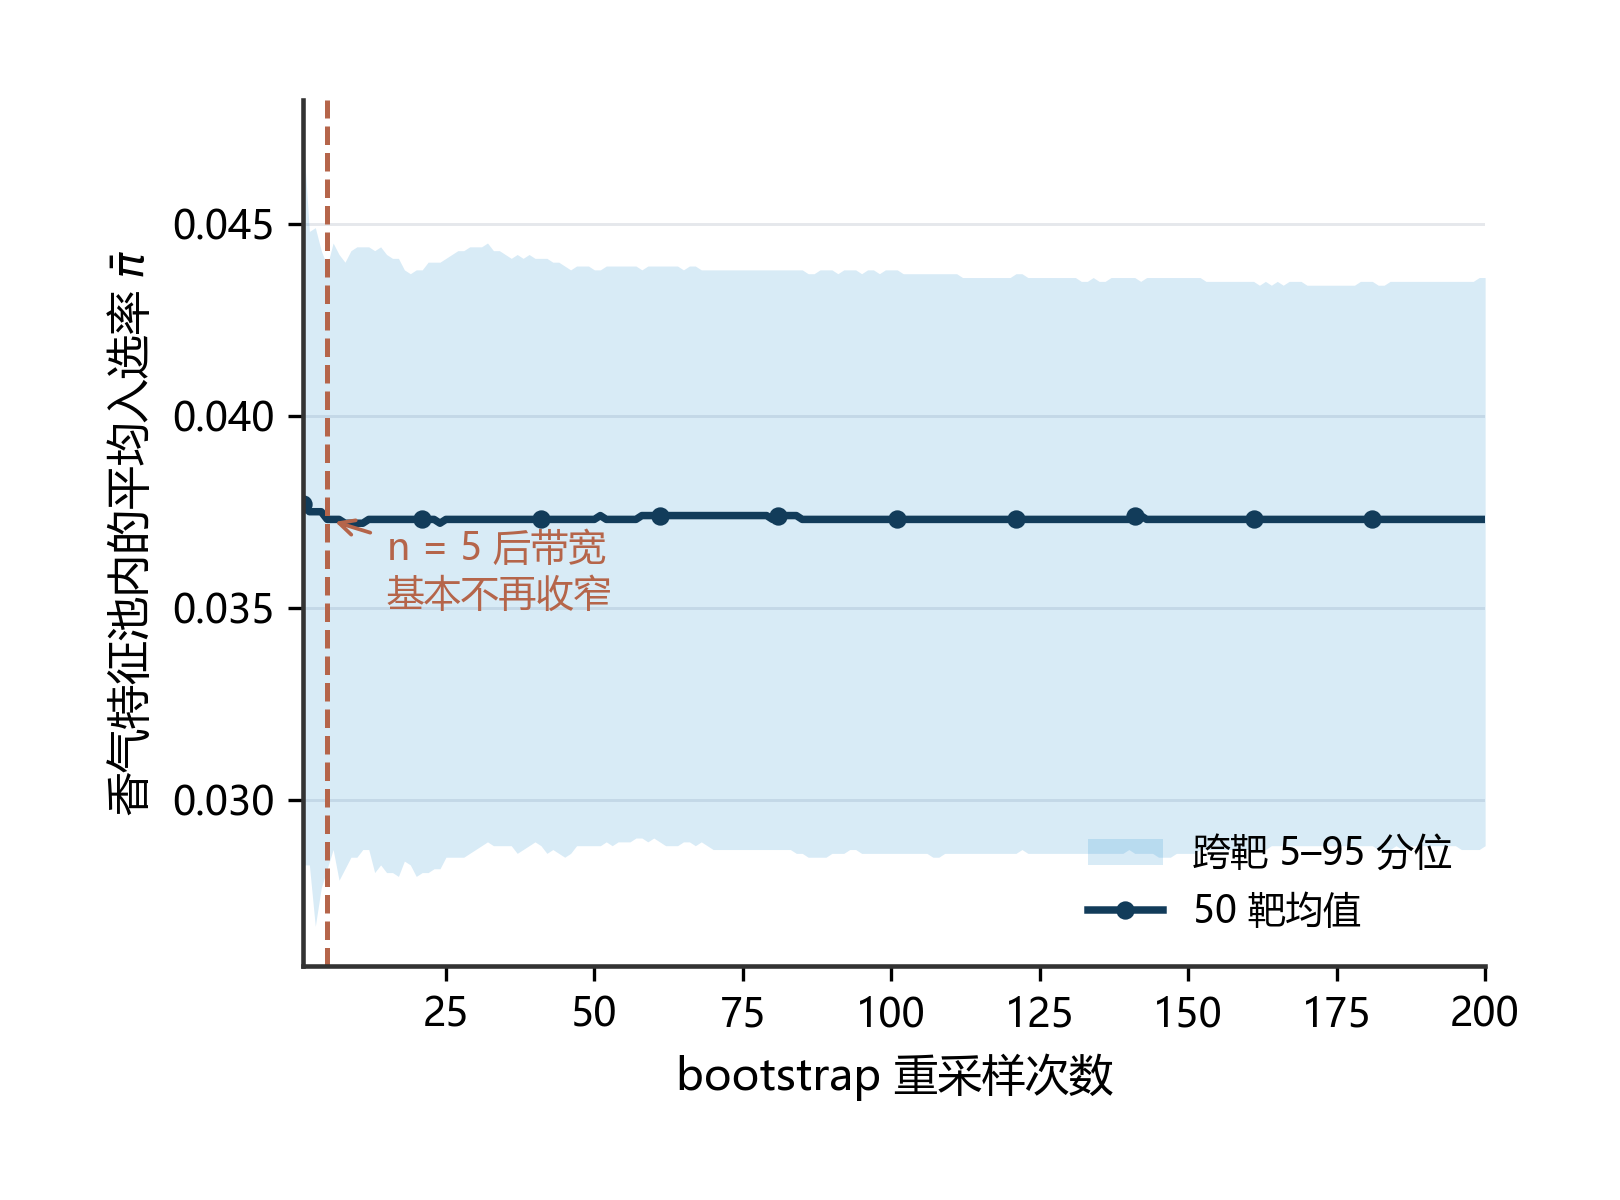
\includegraphics[width=\linewidth]{figures/fig_q2_convergence.png}
\caption{$\pi$ 的自助收敛}
\label{fig:q2conv}
\end{subfigure}
\hfill
\begin{subfigure}[t]{0.48\textwidth}
\centering
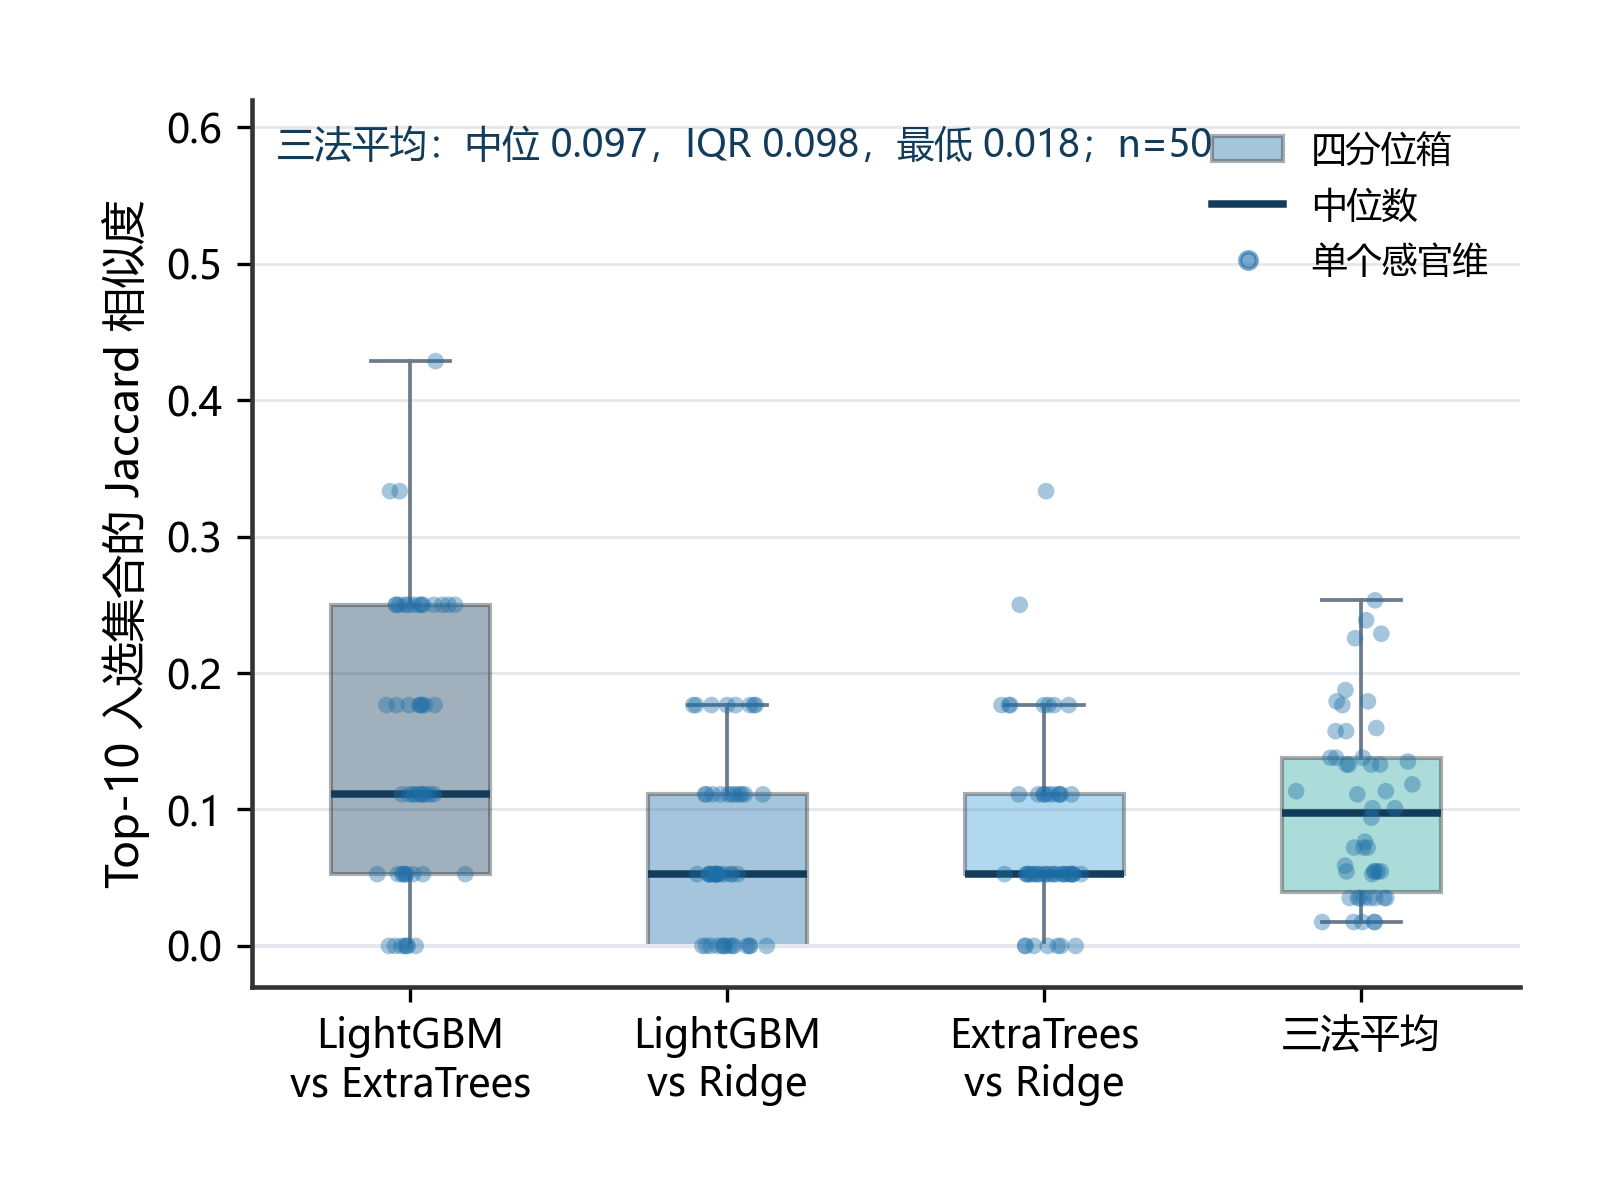
\includegraphics[width=\linewidth]{figures/fig_q2_jaccard.png}
\caption{跨模型 Jaccard 分布}
\label{fig:q2jac}
\end{subfigure}
\caption{稳定性的两项检验。左图为重采样 200 次后增量进入标准误带，说明次数够用；右图为跨模型 Jaccard 分布，中位仅 0.0974，说明名单高度依赖模型族}
\end{figure}

\subsection{结果分析}

231 个化合物中有 46 个在至少一个感官项上超过阈值。150 条 Top-3 记录按阈值能否计算分两条线：67 条有阈值可算 OAV，其中 62 条同时通过 $\pi$ 显著性阈值（$\pi_{\mathrm{thr}}=0.5022$），另 5 条只过 OAV 而不过 $\pi$。四档的分布见表~\ref{tab:q2grade}：A 档 19 条、B 档 8 条、C 档 40 条、N 档 83 条，A+B+C 恰为 67。Top-3 中没有任何理化指标、派生量或内标混入，说明分类规则在前置环节收住了。

\begin{table}[htbp]
\centering
\footnotesize
\caption{问题二 Top-3 记录的证据分级}
\label{tab:q2grade}
\begin{tabular*}{\textwidth}{@{\extracolsep{\fill}}clc}
\toprule
\textbf{档位} & \textbf{判定条件} & \textbf{记录数} \\
\midrule
A & 阈值可算且 $\mathrm{OAV}\geq1$，化学上确可被感知 & 19 \\
B & 阈值可算且 $0.5\leq\mathrm{OAV}<1$，接近阈值 & 8 \\
C & 阈值可算但 $\mathrm{OAV}<0.5$，远离阈值 & 40 \\
N & 阈值缺失（表中无该行，或有行但阈值为 NA），OAV 不可算 & 83 \\
\bottomrule
\end{tabular*}
\end{table}

全部 50 项的 Top-3 名单按能否做化学裁判拆成两张表：表~\ref{tab:q2top3a} 是 A/B 档（至少一个化合物阈值可算且可被闻到），表~\ref{tab:q2top3b} 是 C/N 档（阈值缺失或 OAV 远低于阈值）。表中 $\pi$ 为逐列置换的入选频率，只在同一感官项内可比；末位字母为证据等级，括号内为 OAV 中位数。可以看到 50 项里有 31 项不存在 A 档记录——这不是遗漏，而是阈值表覆盖率不足的直接后果：261 行阈值里只有 43 行有数值，其余留空，注释里本文不把它们称为关键香气化合物。

\begingroup
\scriptsize
\setlength{\tabcolsep}{3.5pt}
\renewcommand{\arraystretch}{1.12}
\begin{longtable}{@{}>{\raggedright\arraybackslash}p{2.7cm}>{\raggedright\arraybackslash}p{4.1cm}>{\raggedright\arraybackslash}p{4.1cm}>{\raggedright\arraybackslash}p{4.1cm}@{}}
\caption{A/B 档：可用阈值做化学裁判的感官项 Top-3。每格第一行为化合物名，第二行为入选频率 $\pi$、证据等级与 OAV 中位数（$>1$ 表示浓度已超其香气阈值）}
\label{tab:q2top3a}\\
\toprule
\textbf{感官项} & \textbf{Top-1} & \textbf{Top-2} & \textbf{Top-3} \\
\midrule
\endfirsthead
\toprule
\textbf{感官项} & \textbf{Top-1} & \textbf{Top-2} & \textbf{Top-3} \\
\midrule
\multicolumn{4}{r@{}}{\footnotesize\itshape 续表~\ref{tab:q2top3a}}\\
\endhead
\bottomrule
\endlastfoot
A\_malt\_cara & octyl\_acetate\newline 0.35C (0.0) & acetic\_acid.\allowbreak g.\allowbreak L.\allowbreak \newline 0.34A (1.2) & furfural\newline 0.32C (0.0) \\
A\_hops\_all & DMS\newline 0.74A (1.4) & ethyl\_octanoate\newline 0.65B (0.7) & X2.\allowbreak 3.\allowbreak dihydro.\allowbreak farnesol\newline 0.34N \\
A\_hops\_tropical & isopentyl.\allowbreak butanoate\newline 0.68N & DMS\newline 0.49A (1.4) & n.\allowbreak hexanol\newline 0.36N \\
A\_hops\_noble & ethyl\_octanoate\newline 0.81B (0.7) & ethyl\_decanoate\newline 0.48C (0.1) & X2.\allowbreak acetylfuran\newline 0.40N \\
A\_esters\_ethac & phenethyl\_alcohol\newline 0.46C (0.2) & ethyl.\allowbreak tetradecanoate\newline 0.43N & ethyl\_acetate\newline 0.41A (1.2) \\
A\_esters\_isoaa & n.\allowbreak hexanol\newline 0.90N & isopentyl\_acetate\newline 0.83A (3.6) & ethyl\_decanoate\newline 0.46C (0.1) \\
F\_hops\_all & ethyl\_octanoate\newline 0.89B (0.7) & cis.\allowbreak dihydro.\allowbreak beta.\allowbreak terpineol\newline 0.68N & DMS\newline 0.52A (1.4) \\
F\_hops\_tropical & n.\allowbreak hexanol\newline 0.56N & nerol.\allowbreak oxide\newline 0.47N & DMS\newline 0.38A (1.4) \\
F\_hops\_noble & ethyl\_octanoate\newline 0.88B (0.7) & citronellol\newline 0.34A (8.8) & nerol.\allowbreak oxide\newline 0.29N \\
F\_esters\_all & n.\allowbreak hexanol\newline 0.67N & ethyl\_acetate\newline 0.66A (1.2) & acetaldehyde\newline 0.65C (0.1) \\
F\_esters\_ethac & ethyl\_acetate\newline 0.81A (1.2) & acetaldehyde\newline 0.47C (0.1) & Z.\allowbreak Z.\allowbreak geranyl.\allowbreak linalool\newline 0.43N \\
F\_esters\_isoaa & isopentyl\_acetate\newline 0.56A (3.6) & ethyl\_decanoate\newline 0.40C (0.1) & delta.\allowbreak terpinyl.\allowbreak acetate\newline 0.34N \\
F\_esters\_fruity & X1.\allowbreak 10.\allowbreak di.\allowbreak epi.\allowbreak cubenol\newline 0.59N & X.\allowbreak E.\allowbreak .\allowbreak alpha.\allowbreak ionone\newline 0.47N & acetic\_acid.\allowbreak g.\allowbreak L.\allowbreak \newline 0.35A (1.2) \\
acidity & lactic\_acid.\allowbreak mg.\allowbreak L.\allowbreak \newline 0.95C (0.3) & ethyl.\allowbreak phenylacetate\newline 0.73N & acetic\_acid.\allowbreak g.\allowbreak L.\allowbreak \newline 0.57A (1.2) \\
bitternes & ethyl\_octanoate\newline 0.94B (0.7) & butyl.\allowbreak acetate\newline 0.69N & ethyl\_decanoate\newline 0.57C (0.1) \\
orange & terpinen.\allowbreak 4.\allowbreak ol\newline 0.78N & geraniol\newline 0.69A (4.4) & ethyl.\allowbreak .\allowbreak E.\allowbreak .\allowbreak linalool\newline 0.57N \\
coriander & camphor\newline 0.86N & geraniol\newline 0.57A (4.4) & ethyl.\allowbreak .\allowbreak E.\allowbreak .\allowbreak linalool\newline 0.56N \\
acetic & lactic\_acid.\allowbreak mg.\allowbreak L.\allowbreak \newline 0.90C (0.3) & ethyl\_isovalerate\newline 0.69C (0.1) & acetic\_acid.\allowbreak g.\allowbreak L.\allowbreak \newline 0.65A (1.2) \\
alcohol & ethyl\_octanoate\newline 0.70B (0.7) & acetaldehyde\newline 0.53C (0.1) & ethyl\_acetate\newline 0.45A (1.2) \\
aftertaste & ethyl\_isovalerate\newline 0.68C (0.1) & acetaldehyde\newline 0.62C (0.1) & ethyl\_octanoate\newline 0.55B (0.7) \\
co2 & ethyl\_octanoate\newline 0.79B (0.7) & nerol\newline 0.69N & ethyl\_hexanoate\newline 0.41A (1.0) \\
overall & X2.\allowbreak ethyl.\allowbreak 1.\allowbreak hexanol\newline 0.47N & cis.\allowbreak linalool.\allowbreak oxide\newline 0.34N & ethyl\_acetate\newline 0.32A (1.2) \\
\end{longtable}
\endgroup



表~\ref{tab:q2top3a} 是被判为 A 档或 B 档的全部感官项——即至少有一个 Top-3 化合物既能算 OAV、又能被闻到。这一组的化学解释可直接给出：$\texttt{A\_malt\_cara}$ 的乙酸与焦糖麦芽香对应美拉德反应产物，$\texttt{A\_hops\_all}$ 的 DMS 与 $\texttt{F\_hops\_all}$ 的辛酸乙酯分别是酒花硫味与果香的主体，$\texttt{lactic}$/$\texttt{acetic}$ 直接对应两种有机酸。

\begingroup
\scriptsize
\setlength{\tabcolsep}{3.5pt}
\renewcommand{\arraystretch}{1.12}
\begin{longtable}{@{}>{\raggedright\arraybackslash}p{2.7cm}>{\raggedright\arraybackslash}p{4.1cm}>{\raggedright\arraybackslash}p{4.1cm}>{\raggedright\arraybackslash}p{4.1cm}@{}}
\caption{C/N 档：阈值缺失或 OAV 远低于阈值的感官项 Top-3。这些记录只作统计候选，不构成关键化合物结论}
\label{tab:q2top3b}\\
\toprule
\textbf{感官项} & \textbf{Top-1} & \textbf{Top-2} & \textbf{Top-3} \\
\midrule
\endfirsthead
\toprule
\textbf{感官项} & \textbf{Top-1} & \textbf{Top-2} & \textbf{Top-3} \\
\midrule
\multicolumn{4}{r@{}}{\footnotesize\itshape 续表~\ref{tab:q2top3b}}\\
\endhead
\bottomrule
\endlastfoot
A\_malt\_all & X2.\allowbreak acetylfuran\newline 0.35N & octyl\_acetate\newline 0.34C (0.0) & X.\allowbreak E.\allowbreak .\allowbreak alpha.\allowbreak ionone\newline 0.26N \\
A\_malt\_grain & X5.\allowbreak methylfurfural\newline 0.51N & terpinen.\allowbreak 4.\allowbreak ol\newline 0.33N & Z.\allowbreak nerolidol\newline 0.32C (0.0) \\
A\_malt\_bread & X2.\allowbreak acetylpyrrole\newline 0.34N & alpha.\allowbreak humulene\newline 0.30C (0.0) & ethyl.\allowbreak tiglate\newline 0.26N \\
A\_malt\_burn & methylpyrazine\newline 0.46C (0.0) & X2.\allowbreak acetylpyrrole\newline 0.23N & ethyl.\allowbreak furoate\newline 0.20N \\
A\_hops\_citrus & isopropyl.\allowbreak tetradecanoate\newline 0.27N & E.\allowbreak caryophyllene\newline 0.26C (0.0) & y.\allowbreak methyl.\allowbreak 1.\allowbreak octanol\newline 0.25N \\
A\_hops\_woody & alloaromadendrene.\allowbreak epoxide\newline 0.61N & X2Z.\allowbreak 6Z.\allowbreak farnesol\newline 0.34N & X1.\allowbreak octen.\allowbreak 3.\allowbreak ol\newline 0.34N \\
A\_esters\_all & n.\allowbreak hexanol\newline 0.92N & lactic\_acid.\allowbreak mg.\allowbreak L.\allowbreak \newline 0.51C (0.3) & acetaldehyde\newline 0.41C (0.1) \\
A\_esters\_flower & ethyl.\allowbreak lactate\newline 0.60N & n.\allowbreak hexanol\newline 0.48N & phenylacetaldehyde\newline 0.40N \\
A\_esters\_fruity & beta.\allowbreak phellandrene\newline 0.85N & X.\allowbreak E.\allowbreak .\allowbreak alpha.\allowbreak ionone\newline 0.54N & delta.\allowbreak terpinyl.\allowbreak acetate\newline 0.34N \\
F\_malt\_all & acetaldehyde\newline 0.63C (0.1) & methylpyrazine\newline 0.49C (0.0) & X.\allowbreak E.\allowbreak .\allowbreak alpha.\allowbreak ionone\newline 0.39N \\
F\_malt\_grain & tau.\allowbreak cadinol\newline 0.41N & n.\allowbreak heptanol\newline 0.38N & ethyl.\allowbreak nicotinate\newline 0.24C (0.0) \\
F\_malt\_bread & X2.\allowbreak acetylpyrrole\newline 0.77N & ethyl.\allowbreak tiglate\newline 0.38N & X2.\allowbreak acetylfuran\newline 0.31N \\
F\_malt\_cara & acetaldehyde\newline 0.70C (0.1) & methylpyrazine\newline 0.39C (0.0) & X.\allowbreak E.\allowbreak .\allowbreak alpha.\allowbreak ionone\newline 0.30N \\
F\_malt\_burn & methylpyrazine\newline 0.39C (0.0) & X2.\allowbreak furanmethanol\newline 0.35N & ethyl.\allowbreak furoate\newline 0.34N \\
F\_hops\_citrus & alpha.\allowbreak terpinyl.\allowbreak isobutanoate\newline 0.38N & ethyl.\allowbreak furoate\newline 0.38N & phenethyl\_alcohol\newline 0.35C (0.2) \\
F\_hops\_woody & isobutanol\newline 0.77C (0.1) & X.\allowbreak E.\allowbreak .\allowbreak 2.\allowbreak nonenal\newline 0.39N & X2.\allowbreak furanmethanol\newline 0.28N \\
F\_esters\_flower & phenylacetaldehyde\newline 0.39N & delta.\allowbreak terpinyl.\allowbreak acetate\newline 0.36N & X2.\allowbreak methyltetrahydrofuran.\allowbreak 3.\allowbreak one\newline 0.34N \\
sweetness & ethyl\_decanoate\newline 0.59C (0.1) & pentyl.\allowbreak octanoate\newline 0.41N & alpha.\allowbreak humulene\newline 0.34C (0.0) \\
X4vg & X4VG\newline 0.98C (0.0) & delta.\allowbreak terpinyl.\allowbreak acetate\newline 0.97N & X14.\allowbreak hydroxy.\allowbreak 9.\allowbreak epi.\allowbreak .\allowbreak E.\allowbreak .\allowbreak caryophyllene\newline 0.41N \\
diacetyl & eugenol\newline 0.96N & lactic\_acid.\allowbreak mg.\allowbreak L.\allowbreak \newline 0.38C (0.3) & octyl\_acetate\newline 0.36C (0.0) \\
dms & E.\allowbreak nerolidol\newline 0.49N & n.\allowbreak decanol\newline 0.41N & terpinen.\allowbreak 4.\allowbreak ol\newline 0.29N \\
metallic & alpha.\allowbreak calacorene\newline 0.48N & Z.\allowbreak Z.\allowbreak geranyl.\allowbreak linalool\newline 0.42N & furfural\newline 0.31C (0.0) \\
stale\_hops & alloaromadendrene.\allowbreak epoxide\newline 0.64N & linalool.\allowbreak isovalerate\newline 0.30N & X2.\allowbreak undecanol\newline 0.28N \\
t2n & vinyl.\allowbreak caprylate\newline 0.38N & ambroxide\newline 0.28N & Z.\allowbreak nerolidol\newline 0.28C (0.0) \\
clove & X4VG\newline 0.63C (0.0) & eucalyptol\newline 0.60N & cis.\allowbreak beta.\allowbreak terpineol\newline 0.58N \\
lactic & lactic\_acid.\allowbreak mg.\allowbreak L.\allowbreak \newline 0.95C (0.3) & ethyl.\allowbreak phenylacetate\newline 0.64N & prenyl.\allowbreak isobutyrate\newline 0.47N \\
barnyard & alloaromadendrene.\allowbreak epoxide\newline 0.59N & linalool.\allowbreak isovalerate\newline 0.35N & n.\allowbreak hexanol\newline 0.34N \\
body & isobutanol\newline 0.57C (0.1) & MeSH\newline 0.49N & propylene.\allowbreak glycol\newline 0.34N \\
\end{longtable}
\endgroup



表~\ref{tab:q2top3b} 的每一项都至少有一个化合物无法完成化学裁判。其中 83 条 N 档记录的原因是阈值表缺失——261 行里只有 43 行有数值；40 条 C 档记录是阈值可算但 OAV 远低于 1。这两类只表示模型依赖，不表示化学因果：例如双乙酰的 Top-1 是丁香酚、DMS 的 Top-1 是 E-橙花叔醇，二者都是 N 档，而双乙酰与 DMS 的已知前体（$\alpha$-乙酰乳酸、S-甲基甲硫氨酸）并未进入 Top-3，原因是共线顶替与阈值缺项。表注中的 $\dagger$ 标记表示该行是目标化合物与特征同名的自相关校验（$\texttt{X4vg}$ 的 Top-1 即 $\texttt{X4VG}$），不计入归因结论。


OAV 的计算结果与酿造学预期一致。图~\ref{fig:q2oav} 给出中位 OAV 最高的化合物：里那醇 13.58、香茅醇 8.79、香叶醇 4.38、乙酸异戊酯 3.62、硫化氢 2.43、DMS 1.40、乙酸乙酯 1.15、己酸乙酯 1.03。前三者均为酒花来源的单萜醇，正是酒花香气的主体；酯类对应果香，DMS 与硫化氢对应硫味与熟蔬菜味，均在文献中有明确描述。

\begin{figure}[htbp]
\centering
\begin{subfigure}[t]{0.48\textwidth}
\centering
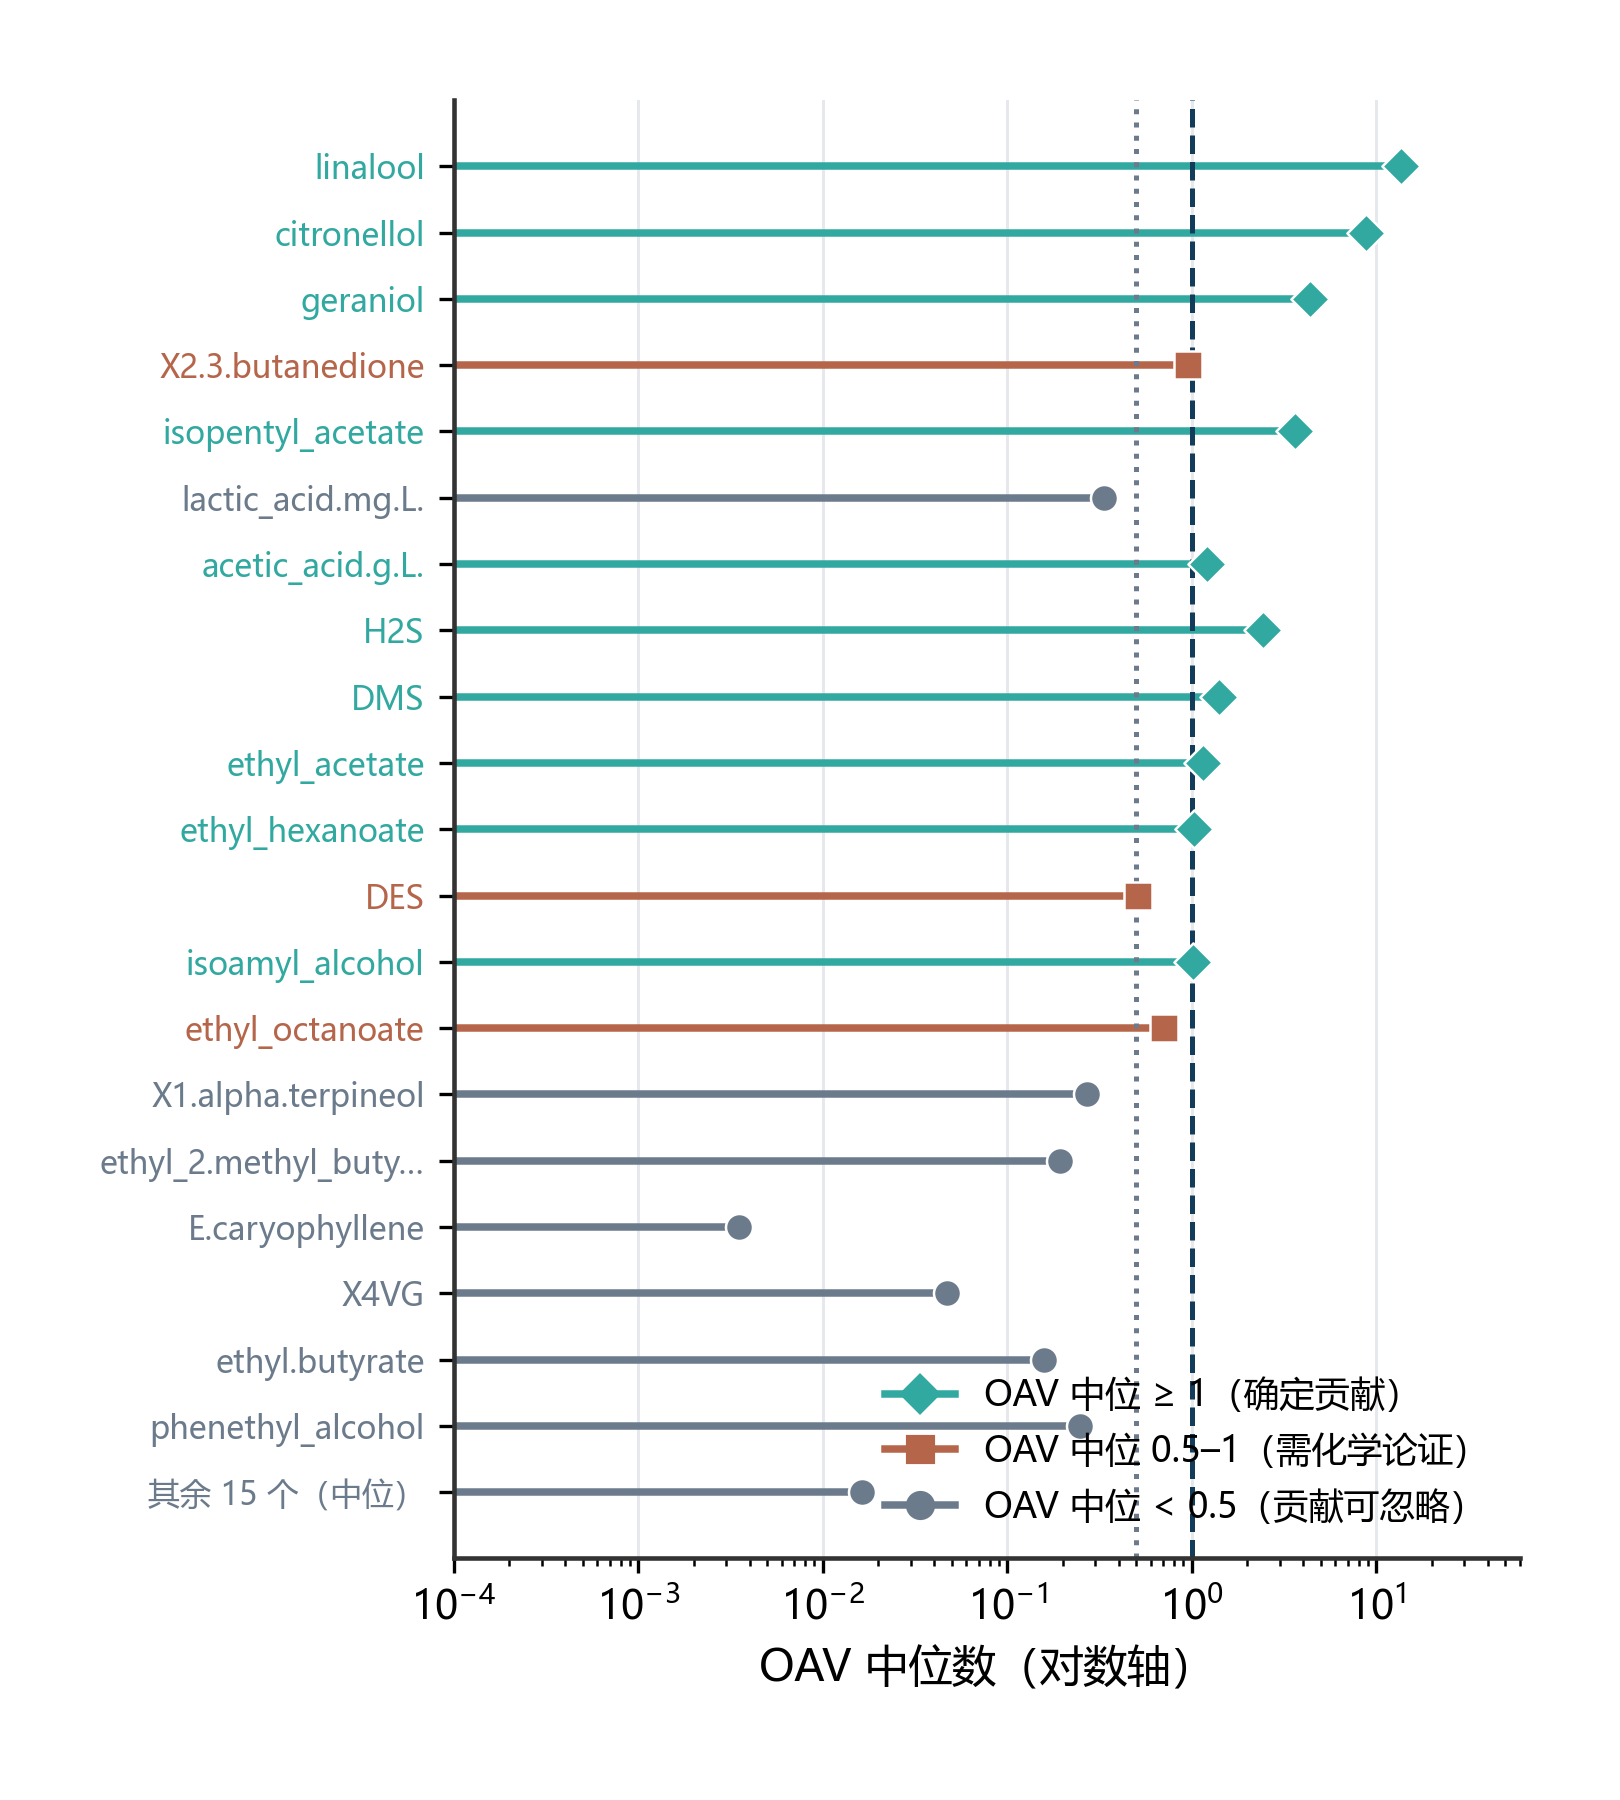
\includegraphics[width=\linewidth]{figures/fig_q2_oav.png}
\caption{化合物 OAV 排序与三档阈值线，纵轴取对数。高于 1 者具备被感知的物质基础}
\label{fig:q2oav}
\end{subfigure}
\hfill
\begin{subfigure}[t]{0.48\textwidth}
\centering
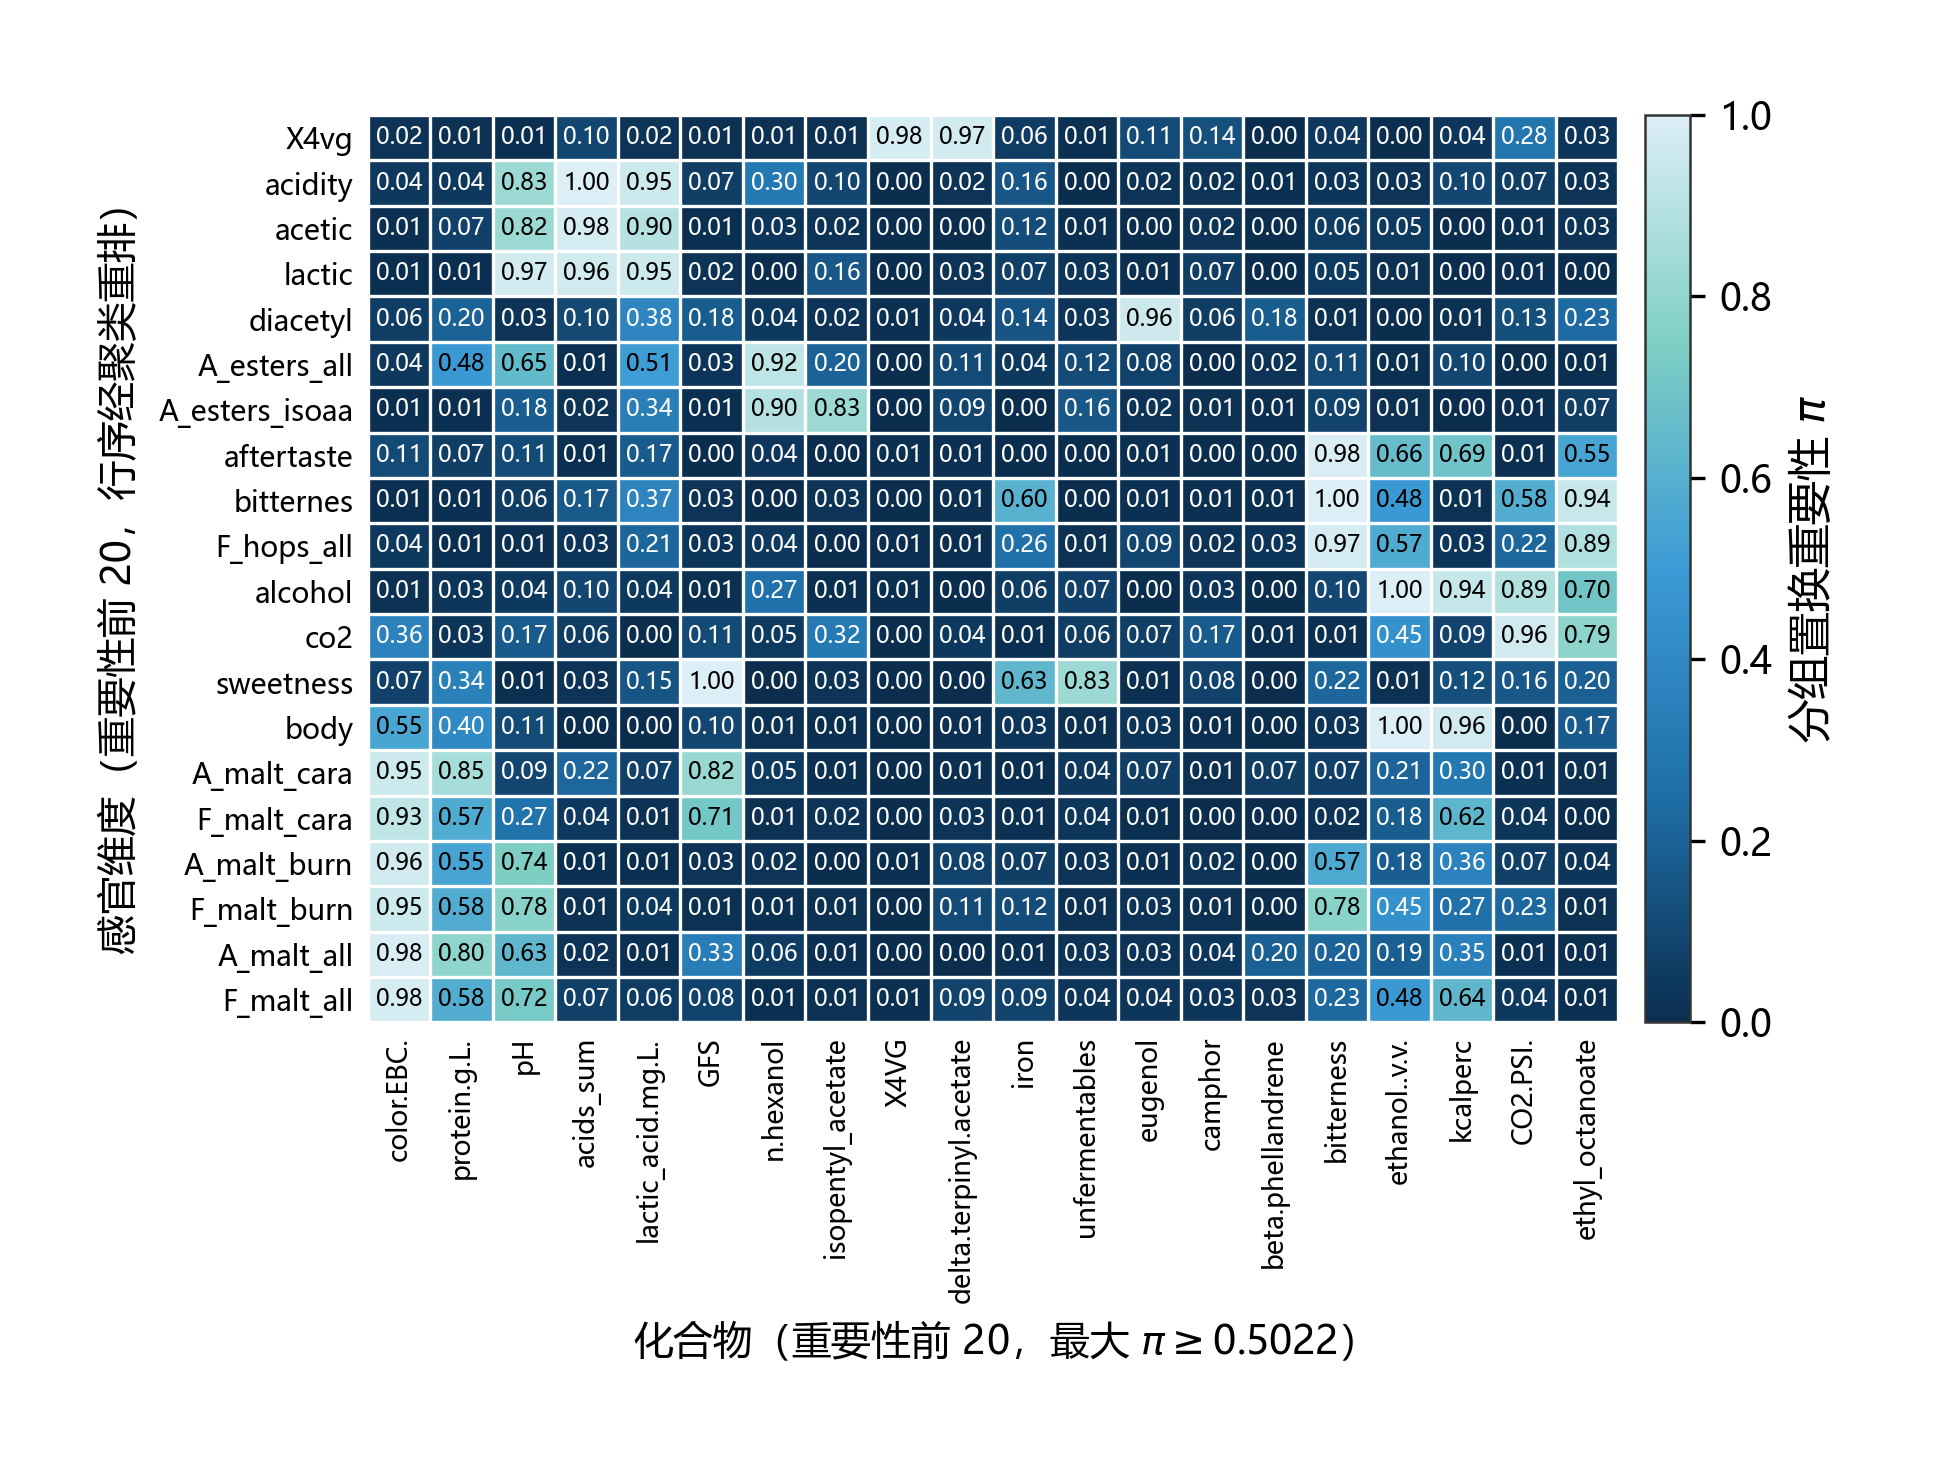
\includegraphics[width=\linewidth]{figures/fig_q2_pi_heatmap.png}
\caption{化合物与感官项的置换重要性矩阵：横轴为 50 个感官项，纵轴为化合物，颜色为 $\pi$ 的大小}
\label{fig:q2heat}
\end{subfigure}
\caption{化学合理性与归因全貌。左图为化合物 OAV 排序与三档阈值线（纵轴取对数），高于 1 者具备被感知的物质基础；右图为置换重要性矩阵}
\end{figure}

图~\ref{fig:q2heat} 给出化合物与感官的置换重要性矩阵：重要性集中于少数几列，其高值区与化学族一一对应。



稳定性是必须如实披露的短板。跨模型 Top-10 的 Jaccard 中位只有 0.0974，四分位距 0.0984，最小 0.0175、最大 0.2533(图~\ref{fig:q2jac})。这说明在 250 个样本、219 列强共线的条件下，Top-3 名单高度依赖模型族。因此本文的交付方式是：只把 A 档 19 条作为统计与化学两个条件的交集报告，C 档 40 条标注为“需额外化学论证”,N 档 83 条不进入结论，并在支撑材料里给出稳定性数值供复核。

逐项不稳定可以用比 Jaccard 更直接的方式量化。200 次重采样给出每个化合物在每个感官项上的平均排名 consrank，1 为最靠前，据此定义“稳定进前 $k$”的子集：以 $k=5$ 计，50 项中有 40 项连一个化合物都凑不出；即使只看每项第 1 名，consrank 中位也高达 11.8。在 250 个样本、219 列强共线的条件下，“每项各选三类关键化合物”本身就不是数据能稳定回答的问题。

因此本文补一条更稳的读法：不逐项选，而是问“哪些化合物在多个感官项上同时稳定靠前”。这个问法要求同一化合物在多个项上同时排名靠前，随机噪声很难同时抬高它在十几个独立拟合中的名次，因此稳定性自然提高。结果见表~\ref{tab:q2consensus}。

\begin{table}[htbp]
\centering
\small
\caption{跨感官项的共识归因，按进入前 5 名的项数降序，列出前 8 位}
\label{tab:q2consensus}
\begin{tabular*}{\textwidth}{@{\extracolsep{\fill}}lcc@{}}
\toprule
\textbf{化合物} & \textbf{前 5 名的项数} & \textbf{前 3 名的项数} \\
\midrule
\texttt{lactic\_acid}（酸感、酯香、酒体） & 13 & 9 \\
\texttt{acetaldehyde}（青苹果、溶剂） & 10 & 10 \\
\texttt{DMS}（熟蔬菜） & 9 & 1 \\
\texttt{phenethyl\_alcohol}（玫瑰花香） & 8 & 6 \\
\texttt{beta.phellandrene}（果香） & 8 & 5 \\
\texttt{prenyl.isobutyrate}（麦芽香） & 7 & 2 \\
\texttt{X1.10.di.epi.cubenol}（果香） & 7 & 6 \\
\texttt{X2.acetylfuran}（焦糖香） & 6 & 4 \\
\bottomrule
\end{tabular*}
\end{table}

这八位的化学解释都站得住：乳酸是酸感的直接物质基础，同时通过 pH 影响酯类的水解速率，因此在酸感、酯香、酒体三类上同时靠前；乙醛是发酵中间产物，带青苹果与溶剂气味，在麦芽香与后味上一致出现；DMS 是熟蔬菜味的缺陷物，但同时会干扰酒花香的判断，因此在前 5 名频繁出现而在前 3 名罕见——这一差异本身就说明它的作用是被“减去”而非“加上”；苯乙醇与辛酸乙酯分别是玫瑰花香与果香的主体，与酿造学一致。

两种读法回答不同的问题：逐项 Top-3 回答“某一感官项的化学来源”，只有 19 条通过双条件；跨项共识回答“整个风味体系的枢纽化合物”，即上表 8 位。前者细而不稳，后者粗而稳，本文并列报告而不偏取其一。

正结果的边界也须说明：统计显著性与预测能力不是同一件事。$R^2$ 最低的若干项如 barnyard 与 stale\_hops，在问题二同样只有很弱的重要性，两问方向一致；反之不成立。
